\chapter{MICROPOL Module}

The MICROPOL module simulates the evolution of a micropollutant (radioelement or heavy metal)
in the three compartments considered to be of major importance in a river ecosystem:
water, Suspended Particulate Matter (SPM) and bottom material.
Each of these compartments represents an homogeneous class:
SPM and sediments represent the grain-size class of clay and silt
(cohesive fine sediments, of diameter about less than 20 to 25 $\mu$m),
likely to attach the majority of micropollutants.\\

Due to adsorption and desorption of micropollutants,
SPM is one of the first links in the chain of contamination.
SPM is carried and dispersed in the water mass
as a tracer and is also subject to the laws of sedimentary physics:
it settles in calm waters and produces bottom sediments,
and can be re-suspended by a high flow.
Deposits cannot move. They are treated as tracers that can be neither advected
nor dispersed by the water mass, but are likely to be re-suspended.\\

The model considers 5 tracers:

\begin{itemize}
\item suspended matter (SS),
\item bottom sediments (SF), neither advected nor dispersed,
\item dissolved form of micropollutant,
\item the fraction adsorbed by suspended particulate matter,
\item the fraction adsorbed by bottom sediments, neither advected nor dispersed.
\end{itemize}

\subsubsection{Notes, and limitations of the MICROPOL module}

\begin{itemize}
\item whether in suspension or deposited on the bottom, the matter is considered
  to be a passive tracer:
  in other words, it does not influence the flow (no feedback).
  This hypothesis involves that the deposits depth must be negligible compared
  to the water depth (the bed is assumed to be unmodified).
\item there is no direct adsorption/desorption of dissolved micropollutants
  on the deposited matter, only on the SPM
  (the model assumes a preponderance of water – SPM exchanges over direct water
  – bottom sediment exchanges).
  Bottom sediments only become radioactive by means of polluted SPM deposition. 
\end{itemize}

\section{Suspended matter}

\subsection{Description of phenomena}

The model describing the evolution of SPM and bottom sediments involved in MICROPOL
is a classic representation of the deposition laws and re-suspension
of cohesive SPM, that are the laws of Krone \cite{krone_flume_1962}
and Partheniades \cite{partheniades_erosion_deposition_1965}.\\

Both processes require the knowledge of characteristic constants:

\begin{itemize}
\item deposition occurs when bottom shear stress $\tau_b$,
  which varies according to the flow conditions, becomes lower than a threshold value $\tau_s$,
  known as the critical shear stress for sedimentation.
  It is then assumed that the SPM settles at a constant velocity $w$
  (known as the settling velocity or velocity of sedimentation),
\item re-suspension occurs when a threshold $\tau_r$,
  known as the critical shear stress for re-suspension, is exceeded.
  Its importance is weighted by a constant $e$, the rate of erosion characteristic
  of deposited SPM (also known as the Partheniades constant).
\end{itemize}

\subsection{Equations}

These phenomena translate into the following expressions of deposition flux ($SED$) and erosion ($RS$),
in kg/m$^2$/s:

\begin{equation}
  SED = \left\{
    \begin{array}{ccl}
      wSS \left( 1 - \frac{\tau_b}{\tau_s} \right) & \rm{if} & \tau_b < \tau_s\\
      0 & \rm{if} & \tau_b \ge \tau_s
    \end{array}
    \right .
\end{equation}

\begin{equation}
  RS = \left\{
    \begin{array}{ccl}
% \varepsilon(SF)
      e \left( \frac{\tau_b}{\tau_r} -1 \right) & \rm{if} & \tau_b > \tau_r\\
      0 & \rm{if} & \tau_b \le \tau_r
    \end{array}
    \right .
\end{equation}

%where $\varepsilon(x)$ is a function such that $\varepsilon(x) = 0$
%if $x = 0$ and $\varepsilon(x) = 1$ else.\\

The bottom shear stress $\tau_b$ (in Pa) is given by $\tau_b = \frac{1}{2} \rho C_f U^2$,
with $C_f$ = the friction coefficient and $U^2$ the square of the velocity.\\

The equations of the evolution of SPM tracers (variable $SS$)
and bottom sediments (variable $SF$) are as follows:\\

Tracer $\#$1: suspended particulate matter

\begin{equation}
  F(SS) = \frac{RS-SED}{h}.
\end{equation}

Tracer $\#$2: bottom sediments (tracer neither advected nor diffused)\\

\begin{equation}
  \frac{\partial (SF)}{\partial t} = SED - RS.
\end{equation}

The model relating to SPM has four parameters: the velocity of sedimentation $w$,
the erosion rate $e$, the critical shear stress for deposition $\tau_s$
and the critical shear stress for erosion $\tau_r$.

\section{Micropollutants}

\subsection{Description of phenomena}

The model representing the evolution of micropollutants assumes
that the transfers of micropollutants (radioelement, metal)
between the dissolved and particulate phases correspond to either
direct adsorption or ionic exchanges modeled by a reversible reaction,
of 1$^{\rm{st}}$ kinetic order \cite{ciffroy_doubs_1995}.
In the case of direct adsorption, the reaction can be represented in the form of the following formula:\\

\begin{figure}[H]
  \centering
  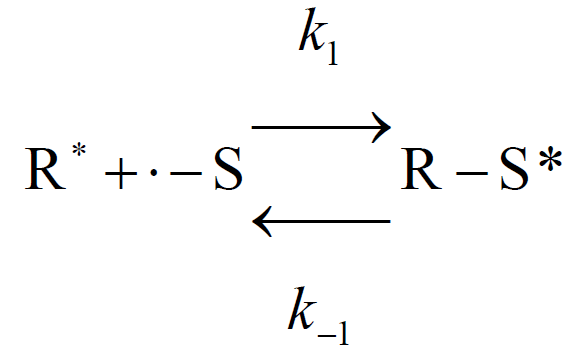
\includegraphics[scale=0.4]{graphics/image60.png}
\end{figure}

%$R^\ast +.- S    k_1/k_{-1}     R - S^\ast$

with R$^\ast$ = micropollutant in dissolved form, – S = surface site associated with SPM,
R–S$^{\ast}$ = adsorbed micropollutant.\\

It is a reversible reaction, controlled by adsorption ($k_1$ in l/g/s)
and desorption velocities ($k_{-1}$ in s$^{-1}$).
It leads to an equilibrium state, and then a distribution of micropollutants
between the dissolved and particulate phase described
by the distribution coefficient $K_d$ (in l/g):

\begin{equation}
  K_d = \frac{[R-S^\ast]}{[R^\ast]} = \frac{k_1}{k_{-1}},
\end{equation}

where [R$^\ast$] is the activity (or concentration of micropollutant)
in dissolved phase (in Bq/m$^3$ or kg/m$^3$), [R-S$^\ast$] is the activity
(or concentration of micropollutant) associated to SPM (in Bq/kg or kg/kg).\\

Once adsorbed, the fixed micropollutants act like SPM (deposition, re-suspension)
and can also produce areas of polluted sediment.\\

The model includes an exponential decay law (radioactive decay type) of micropollutant
concentrations in each compartment of the modeled ecosystem,
through a constant written $L$ (expressed in s$^{-1}$).\\

\subsection{Equations}

The system includes an equation for each micropollutant phase, namely 3 tracers:

\begin{itemize}
\item $C$: concentration of micropollutants in water (Bq/m$^3$),
\item $C_s$: concentration of micropollutants adsorbed by SPM (Bq/kg) (dry weight),
\item $C_f$: concentration of micropollutants adsorbed by bottom sediments (Bq/kg).
\end{itemize}

Note: The unit of concentration chosen for the demonstration is Bq/m$^3$,
but it could also be written in kg/m$^3$ (for example, in the case of a metal).\\

The internal sources of each of these tracers correspond to the phenomena
of adsorption/desorption, deposition/re-suspension and exponential decay.
Taking these phenomena into account leads to the following equations
in each of the three compartments, water, SPM and bottom sediments
(with section \ref{waq_models} notations):

\begin{itemize}
\item dissolution phase
\begin{equation}
  F(C) = -k_{-1}.SS (K_d.C - C_s ) - L.C,
\end{equation}

\item adsorption by suspended particulate matter phase
\begin{equation}
  F(SS.C_s) = k_{-1}.SS (K_d.C - C_s ) + \frac{RS.C_f-SED.C_s}{h} - L.SS.C_s,
\end{equation}

\item adsorption by bottom sediments (tracer neither advected nor diffused)
\begin{equation}
  \frac{\partial (SF.C_f)}{\partial t} = SED.C_s - RS.C_f - L.SF.C_f.
\end{equation}

\end{itemize}

Setting the new variables as: $C_{ss}$  = $SS.C_s$, in Bq/m$^3$ of water,
$C_{ff} = SF.C_f$, in Bq/m$^2$ of bottom sediments,
and $SEDP = \frac{SED}{SS} = w \left (1-\frac{\tau_b}{\tau_s} \right)$
if $\tau_b < \tau_s$ or 0 otherwise, the equations become:\\

Tracer $\#$3: dissolution phase

\begin{equation}
  F(C) = -k_{-1}.SS.K_d.C + k_{-1}.C_{SS} - L.C.
\end{equation}

Tracer $\#$4: phase of adsorption by suspended particulate matter

\begin{equation}
  F(C_{SS}) = k_{-1}.K_d.SS.C - k_{-1}.C_{SS} + \frac{\frac{RS}{SF}C_{ff}-SEDP.C_{SS}}{h}- L.C_{SS}.
\end{equation}

Tracer $\#$5: phase of adsorption by bottom sediments

\begin{equation}
  \frac{\partial C_{ff}}{\partial t} = SEDP.C_{SS} - \frac{RS}{SF} C_{ff} - L.C_{ff}.
\end{equation}

Terms with $SF$ as denominator are nullified when $SF$ is equal to 0.\\

Therefore, there are three parameters of the micropollutant model:
the distribution coefficient at equilibrium $K_d$,
the kinetic constant of desorption $k_{-1}$,
and the exponential decay constant $L$ (radioactive decay, for example).
In total, the MICROPOL model includes 7 physical parameters.

\section{Solved equations}

Noting $C_1 = SS$, $C_2 = SF$, $C_3 =C$, $C_4 = C_{ss}$, $C_5 = C_{ff}$ ,
the matrices (5 $\times$ 5) $[\lambda]$ and $[\mu]$
%containing the coefficients $\lambda_i^j$ and $\mu_i^j$
are written as:

$$  \lambda = 
  \begin{pmatrix}
    0 & 0 & 0 & 0 & 0\\
    SEDP & 0 & 0 & 0 & 0\\
    0 & 0 & -L -k_{-1}.SS.K_d & k_{-1} & 0\\
    0 & 0 & -k_{-1}.K_d.SS & -k_{-1} - L & 0\\
    0 & 0 & 0 & SEDP & -\frac{RS}{SF}-L
  \end{pmatrix}
$$  

$$  \mu = 
  \begin{pmatrix}
    -SEDP & 0 & 0 & 0 & 0\\
    0 & 0 & 0 & 0 & 0\\
    0 & 0 & 0 & 0 & 0\\
    0 & 0 & 0 & -SEDP & \frac{RS}{SF}\\
    0 & 0 & 0 & 0 & 0
  \end{pmatrix}
$$  

Note the case where $SF$ = 0: $C_{ff} = 0$, $\lambda_5^5 = 0$ and $\mu_4^5 = 0$.
The only non-zero terms $\lambda_i^0$ and $\mu_i^0$ are $\lambda_2^0 = -RS$ and $\mu_2^0 = RS$.
